\documentclass[a4paper,11pt]{article}
\usepackage{amsmath,amsthm,amsfonts,amssymb,amscd,amstext,vmargin,graphics,graphicx,tabularx,multicol} \usepackage[french]{babel}
\usepackage[utf8]{inputenc}  
\usepackage[T1]{fontenc} 
\usepackage[T1]{fontenc}
\usepackage{amsmath,amssymb}
\usepackage{pstricks-add,tikz,tkz-tab,variations}
\usepackage[autolanguage,np]{numprint} 

\setmarginsrb{1.5cm}{0.5cm}{1cm}{0.5cm}{0cm}{0cm}{0cm}{0cm} %Gauche, haut, droite, haut
\newcounter{numexo}
\newcommand{\exo}[1]{\stepcounter{numexo}\noindent{\bf Exercice~\thenumexo} : \marginpar{\hfill /#1}}
\reversemarginpar


\newcounter{enumtabi}
\newcounter{enumtaba}
\newcommand{\q}{\stepcounter{enumtabi} \theenumtabi.  }
\newcommand{\qa}{\stepcounter{enumtaba} (\alph{enumtaba}) }
\newcommand{\initq}{\setcounter{enumtabi}{0}}
\newcommand{\initqa}{\setcounter{enumtaba}{0}}

\newcommand{\be}{\begin{enumerate}}
\newcommand{\ee}{\end{enumerate}}
\newcommand{\bi}{\begin{itemize}}
\newcommand{\ei}{\end{itemize}}
\newcommand{\bp}{\begin{pspicture*}}
\newcommand{\ep}{\end{pspicture*}}
\newcommand{\bt}{\begin{tabular}}
\newcommand{\et}{\end{tabular}}
\renewcommand{\tabularxcolumn}[1]{>{\centering}m{#1}} %(colonne m{} centrée, au lieu de p par défault) 
\newcommand{\tnl}{\tabularnewline}

\newcommand{\trait}{\noindent \rule{\linewidth}{0.2mm}}
\newcommand{\hs}[1]{\hspace{#1}}
\newcommand{\vs}[1]{\vspace{#1}}

\newcommand{\N}{\mathbb{N}}
\newcommand{\Z}{\mathbb{Z}}
\newcommand{\R}{\mathbb{R}}
\newcommand{\C}{\mathbb{C}}
\newcommand{\Dcal}{\mathcal{D}}
\newcommand{\Ccal}{\mathcal{C}}
\newcommand{\mc}{\mathcal}

\newcommand{\vect}[1]{\overrightarrow{#1}}
\newcommand{\ds}{\displaystyle}
\newcommand{\eq}{\quad \Leftrightarrow \quad}
\newcommand{\vecti}{\vec{\imath}}
\newcommand{\vectj}{\vec{\jmath}}
\newcommand{\Oij}{(O;\vec{\imath}, \vec{\jmath})}
\newcommand{\OIJ}{(O;I,J)}

\newcommand{\bmul}[1]{\begin{multicols}{#1}}
\newcommand{\emul}{\end{multicols}}


\newcommand{\reponse}[1][1]{%
\multido{}{#1}{\makebox[\linewidth]{\rule[0pt]{0pt}{20pt}\dotfill}
}}

\newcommand{\titre}[5] 
% #1: titre #2: haut gauche #3: bas gauche #4: haut droite #5: bas droite
{
\noindent #2 \hfill #4 \\
#3 \hfill #5

\vspace{-1.6cm}

\begin{center}\rule{6cm}{0.5mm}\end{center}
\vspace{0.2cm}
\begin{center}{\large{\textbf{#1}}}\end{center}
\begin{center}\rule{6cm}{0.5mm}\end{center}
}



\begin{document}
\pagestyle{empty}
\titre{Interrogation : Parallélogrammes particuliers}{Nom :}{Prénom :}{Classe}{Date}


\exo{1} À l'aide du codage et \textbf{sans justification}, indiquer la nature de chaque quadrilatère.\\

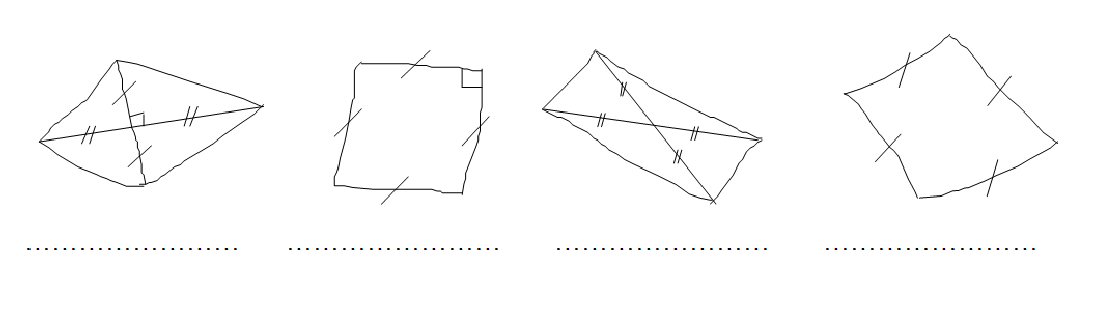
\includegraphics[scale=1]{interro1.eps} 

\exo{3}

\q Construire un losange FGVC tel que : CG = 4 cm  et  FV = 7 cm \\

\vspace*{5cm}


\q Construire un rectangle un rectangle RECT tel que :  RE = 4 cm  et RC = 5 cm.\\

\vspace*{5cm}

\q Construire un carré EFGH tel que : EG = 8cm.\\

\vspace*{7cm}


\newpage

\exo{4,5} Vrai ou Faux\\

\qa Si le quadrilatère EFGH est un parallélogramme, alors : EF = GH   et   EH = FG : ...............\\

\qa Si les segments [EF] et [ZK] ont le même milieu, alors EZFK est un parallélogramme : ...............\\

\qa Un quadrilatère dont les diagonales ont la même longueur, est un rectangle :...............\\

\qa Un rectangle est un parallélogramme : ...............\\

\qa Un parallélogramme dont les diagonales sont perpendiculaires est un losange : ...............\\

\qa Un rectangle a un centre de symétrie et deux axes de symétrie, ses diagonales : ...............\\

\qa Un parallélogramme est un losange : ...............\\

\qa Un parallélogramme qui a un angle doit est un rectangle : ...............\\

\qa Un quadrilatère qui a ses 4 côtés de même longueur est un carré : ............... \\


\exo{4}

\initqa \qa Tracer un triangle RST tel que : 	SR = 3,5 cm	,   RST = 40 degrés   et   SRT = 100 degrés.\\
Placer le point O, milieu du segment [ST].\\
Placer le point U, symétrique de R par rapport à O.\\

\vspace*{5cm}

\qa Démontrer que le quadrilatère SRTU est un parallélogramme.\\
\reponse[3]\\

\qa Calculer la mesure de l'angle $\widehat{RTS}$. Que peut-on alors dire des longueurs RS et RT ? Pourquoi ?\\
\reponse[3]\\

\qa En déduire la nature précise du quadrilatère SRTU.\\
\reponse[3]\\





\end{document}
